\documentclass[tikz,border=3.14pt]{standalone}
\usepackage{../mymacros}
\usepackage{tikz-3dplot}
\usetikzlibrary{fadings}

\definecolor{poliblue1}{RGB}{93,138,168} 
\definecolor{poliblue2}{RGB}{41,76,113}
\definecolor{poliblue3}{RGB}{25,43,67}
\definecolor{orangep}{RGB}{251,146,116}

\begin{document}
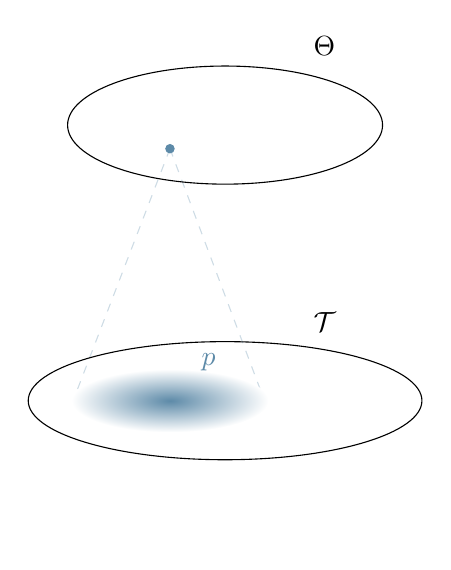
\begin{tikzpicture}[]
\draw[dashed, color=poliblue1, opacity=0.3] (-0.7,-0.3,0) -- (-1.93,-3.5,0);
\draw[dashed, color=poliblue1, opacity=0.3] (-0.7,-0.3,0) -- (0.5,-3.5,0);
\draw[] (0,0,0) ellipse (2 and .75) node[right, shift={(1,1)}]{$\Theta$};
\draw [fill, color=poliblue1] (-0.7,-0.3,0) circle (1.5pt) node[above](a){$\vtheta$};
\draw[] (0,-3.5,0) ellipse (2.5 and .75) node[right, shift={(1,1)}]{$\mathcal{T}$};
\draw[fill, inner color=poliblue1, outer color=white, draw=none, color=white] (-0.7,-3.5,0) ellipse (1.25 and .4) node[above, shift={(.5,.25)}, color=poliblue1]{$p_{\vtheta}$};

\phantom{
\draw [fill, color=black] (-1.1,-3.6,0) circle (1.5pt) node[above](b){$\tau$};
\draw[] (-1.1,-5,0) node (c) {$R(\tau)$};
\draw[->] (b) -- (c);
}
\phantom{\draw[color=poliblue1] (-0.7,-5,0) node (c) {$J(\vtheta)$};}
\end{tikzpicture}
\end{document}